\documentclass{article}
\usepackage{polski}
\usepackage[utf8]{inputenc}
\usepackage{graphicx}
\title{Całki}
\begin{document}
\maketitle
\tableofcontents
\section{Całka}
Ogólne określenie wielu różnych, choć powiązanych ze sobą pojęć analizy matematycznej. Najczęściej przez całkę rozumie się całkę oznaczoną lub całkę nieoznaczoną, choć istnieje wiele innych odmian całki.
\section{Całka nieoznaczona}
Przez całkę nieoznaczoną (albo funkcję pierwotną) rozumie się pojęcie odwrotne do pochodnej funkcji. Całkę oznaczoną na przedziale [a,b] można też zdefiniować (tzw. całka Newtona-Leibniza) jako różnicę między wartościami całki nieoznaczonej w punktach b oraz a. Stąd obliczenie całki nieoznaczonej jest często pierwszym krokiem przy obliczaniu całek oznaczonych.

Uogólnieniem całki nieoznaczonej jest całka równania różniczkowego będąca rozwiązaniem równania różniczkowego: $F'(x)=f(x)$, gdzie $F(x)$ jest pierwotną, $f(x)$ a oznacza całkowaną funkcję.
\section{Całka oznaczona}
Intuicyjnie całka oznaczona to pole powierzchni między wykresem funkcji $f(x)$ w pewnym przedziale $[a,b]$, a osią odciętych, wzięte ze znakiem plus dla dodatnich wartości funkcji i minus dla ujemnych. Pojęcie całki oznaczonej, choć intuicyjnie proste, może być sformalizowane na wiele sposobów. Jeśli jakaś funkcja jest całkowalna według dwóch różnych definicji całki oznaczonej, wynik całkowania będzie taki sam.

\begin{figure}
\caption{Interpretacja graficzna całki oznaczonej}
\label{fig:interpretacja}
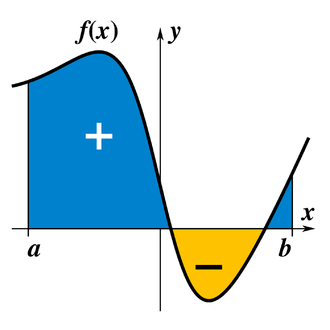
\includegraphics[scale=1.5]{calka1.png}
\centering
\end{figure}

Całkę oznaczoną na przedziale $[a, b]$ z funkcji $f$, można Należy zauważyć, że istnieje też inna definicja, w której powyższe całki są mnożone funkcji $f$ oraz osią $x$: części nad osią oraz pod nią (rysunek \ref{fig:interpretacja}).

\begin{figure}
\caption{Wykres całek Fresnela}
\label{fig:fresnel}
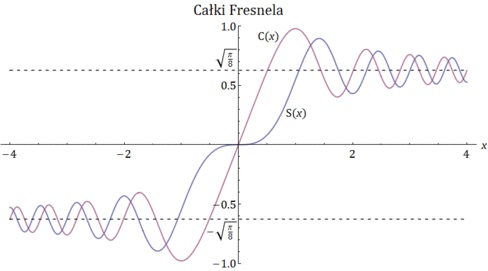
\includegraphics[scale=0.6]{calka2.png}
\centering
\end{figure}

Całki Fresnela- dwie funkcje specjalne $S(x)$ i $C(x)$, zwane odpowiednio sinusem i cosinusem Fresnela (rysunek \ref{fig:fresnel}).

\end{document}